% !TEX encoding = UTF-8 Unicode
\documentclass[a4paper]{article}

\usepackage{color}
\usepackage{url}
\usepackage[T2A]{fontenc} % enable Cyrillic fonts
\usepackage[utf8]{inputenc} % make weird characters work
\usepackage{graphicx}
\usepackage{cite}
\usepackage{amsmath}

\usepackage[english,serbian]{babel}
%\usepackage[english,serbianc]{babel} %ukljuciti babel sa ovim opcijama, umesto gornjim, ukoliko se koristi cirilica

\usepackage[unicode]{hyperref}
\hypersetup{colorlinks,citecolor=green,filecolor=green,linkcolor=blue,urlcolor=blue}

\usepackage{listings}

%\newtheorem{primer}{Пример}[section] %ćirilični primer
\newtheorem{primer}{Primer}[section]

\definecolor{mygreen}{rgb}{0,0.6,0}
\definecolor{mygray}{rgb}{0.5,0.5,0.5}
\definecolor{mymauve}{rgb}{0.58,0,0.82}

\lstset{ 
  backgroundcolor=\color{white},   % choose the background color; you must add \usepackage{color} or \usepackage{xcolor}; should come as last argument
  basicstyle=\scriptsize\ttfamily,        % the size of the fonts that are used for the code
  breakatwhitespace=false,         % sets if automatic breaks should only happen at whitespace
  breaklines=true,                 % sets automatic line breaking
  captionpos=b,                    % sets the caption-position to bottom
  commentstyle=\color{mygreen},    % comment style
  deletekeywords={...},            % if you want to delete keywords from the given language
  escapeinside={\%*}{*)},          % if you want to add LaTeX within your code
  extendedchars=true,              % lets you use non-ASCII characters; for 8-bits encodings only, does not work with UTF-8
  firstnumber=1000,                % start line enumeration with line 1000
  frame=single,	                   % adds a frame around the code
  keepspaces=true,                 % keeps spaces in text, useful for keeping indentation of code (possibly needs columns=flexible)
  keywordstyle=\color{blue},       % keyword style
  language=Python,                 % the language of the code
  morekeywords={*,...},            % if you want to add more keywords to the set
  numbers=left,                    % where to put the line-numbers; possible values are (none, left, right)
  numbersep=5pt,                   % how far the line-numbers are from the code
  numberstyle=\tiny\color{mygray}, % the style that is used for the line-numbers
  rulecolor=\color{black},         % if not set, the frame-color may be changed on line-breaks within not-black text (e.g. comments (green here))
  showspaces=false,                % show spaces everywhere adding particular underscores; it overrides 'showstringspaces'
  showstringspaces=false,          % underline spaces within strings only
  showtabs=false,                  % show tabs within strings adding particular underscores
  stepnumber=2,                    % the step between two line-numbers. If it's 1, each line will be numbered
  stringstyle=\color{mymauve},     % string literal style
  tabsize=2,	                   % sets default tabsize to 2 spaces
  title=\lstname                   % show the filename of files included with \lstinputlisting; also try caption instead of title
}

\begin{document}

\title{Igrajući linkovi\\ \small{Seminarski rad u okviru kursa\\Konstrukcija i Analiza algoritama 2\\ Matematički fakultet}}

\author{Petar Đorđević}

%\date{9.~april 2015.}

\maketitle

\abstract{
  Ovaj rad istražuje Algoritam igrajućih linkova ({\em Dancing Links Algorithm - DLX}),
  koji je efikasna metoda za rešavanje problema pokrivanja tačaka, specifično za
  rešavanje problema tačnog omotača. Algoritam, koji je osmislio Donald
  Knut \cite{knuth2000dancing}, omogućava brzu i efikasnu manipulaciju matrica
  pokrivanja. Ova tehnika je naročito pogodna za rešavanje složenih kombinatornih
  problema kao što je raspoređivanje poslova, logičke  rešetke, puzzle i slično.
  U okviru ovog rada, implementiraće se Sudoku rešavač kao konkretan primer primene 
  Algoritma igrajućih linkova (DLX).

\tableofcontents

\newpage

\section{Uvod}
\label{sec:uvod}
Problem tačnog pokrivača ({\em Exact Cover Problem}) je klasičan kombinatorni problem odabira podskupova
iz date kolekcije tako da svaki element univerzalnog skupa bude tačno jednom pokriven \cite{cover}.
Rešavanje ovog problema ima primenu u raznim oblastima kao što su teorija grafova, optimizacija,
veštačka inteligencija i računarstvo. Problem tačnog pokrivača je NP-težak, što znači da je izuzetno
složen za rešavanje, te zahteva najbolji mogući algoritam za efikasno pronalaženje rešenja.

Jedan od najpoznatijih algoritama za rešavanje ovih problema je Algoritam
igrajućih linkova ({\em Dancing Links Algorithm - DLX}), koji je osmislio Donald Knuth. DLX
koristi strukturu podataka poznatu kao igrajući linkovi koja optimizuje operacije
dodavanja, uklanjanja i pretraživanja elemenata u matricama pokrivanja.

Sudoku je popularna logička slagalica koja zahteva popunjavanje 9x9 mreže brojevima od 1 do 9,
uz poštovanje pravila da se svaki broj mora pojaviti tačno jednom u svakom redu, koloni i 3x3
podmreži. Problem rešavanja Sudokua može se preformulisati kao problem tačnih pokrivača, što ga
čini idealnim za primenu DLX-a. Ovo preformulisanje omogućava da se koristi DLX za efikasno
pronalaženje rešenja, čak i za najteže zagonetke.

Cilj ovog rada je da implementira Sudoku rešavač koristeći Algoritam igrajućih linkova i da
demonstrira efikasnost ovog algoritma. Pored toga, rad će evaluirati performanse DLX-a na
različitim primerima Sudoku zagonetki.

\section{Problem tačnog omotača}

Problem tačnog pokrivača ({\em Exact Cover Problem - ECP}) predstavlja ključnu podvrstu problema
zadovoljivosti ograničenja ({\em Constraint Satisfaction Problems - CSP}), gde je cilj
pronalaženje podskupa elemenata koji tačno pokrivaju dati skup. Svaki podskup se može posmatrati
kao klauza, a tačno pokrivanje zahteva da svaka klauza bude zadovoljena tačno jednom.

ECP se može definisati na sledeći način: Dat je univerzalni skup \( U \)
i kolekcija \( S \) podskupova \( U \). Cilj je pronaći podskup \( S' \subseteq S \) takav
da su svi elementi iz \( U \) tačno jednom pokriveni, odnosno svaki element iz \( U \) pripada
tačno jednom podskupu iz \( S' \).

\[
\mathcal{S}' \subseteq \mathcal{S} \quad \wedge \quad \left( \forall S_1, S_2 \in \mathcal{S}', \ S_1 \neq S_2 \implies S_1 \cap S_2 = \emptyset \right) \quad \wedge \quad \bigsqcup_{S' \in \mathcal{S}'} S' = U
\]

Pošto se ECP može redukovati na CSP probleme \cite{reduction} znamo da je to NP-težak problem,
što i ima smisla intuitivno: da bi se utvrdilo da li dati skup podskupova sadrži tačno pokrivanje,
potrebno je proveriti sve moguće kombinacije, što može dovesti do eksponencijalnog rasta vremena izvršavanja.

Postoje različiti pristupi rešavanju ECP-a, među kojima su i algoritmi koji koriste tehniku pretraživanja
unazad, kao što su algoritam tačne pretrage i algoritam podeli pa vladaj. Pored toga, neki od najefikasnijih
algoritama za rešavanje problema tačnog pokrivača su bazirani na pretraživanju uz upotrebu heuristika, kao
što su gramzivi algoritmi i algoritmi zasnovani na tačnom pokrivanju kontraprimera ({\em backtracking}).
Ovi algoritmi kombinuju preciznost i efikasnost kako bi pronašli optimalna rešenja ili dobra približna rešenja
problema tačnog pokrivača.

\section{Slike i tabele}
\label{slike_i_tabele}

Slike i tabele treba da budu u svom okruženju, sa odgovarajućim naslovima, obeležene labelom da koje omogućava referenciranje. 

\begin{primer} Ovako se ubacuje slika. Obratiti pažnju da je dodato i 
\begin{verbatim}
\usepackage{graphicx}
\end{verbatim}

\begin{figure}[h!]
\begin{center}
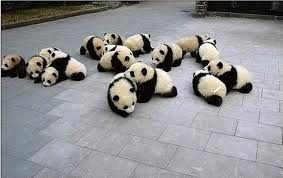
\includegraphics[scale=0.75]{panda.jpg}
\end{center}
\caption{Pande}
\label{fig:pande}
\end{figure}

Na svaku sliku neophodno je referisati se negde u tekstu. Na primer, na slici \ref{fig:pande} prikazane su pande. 
\end{primer}

\begin{primer} I tabele treba da budu u svom okruženju, i na njih je neophodno referisati se u tekstu. Na primer, u tabeli \ref{tab:tabela1} su prikazana različita poravnanja u tabelama.

\begin{table}[h!]
\begin{center}
\caption{Razlčita poravnanja u okviru iste tabele ne treba koristiti jer su nepregledna.}
\begin{tabular}{|c|l|r|} \hline
centralno poravnanje& levo poravnanje& desno poravnanje\\ \hline
a &b&c\\ \hline
d &e&f\\ \hline
\end{tabular}
\label{tab:tabela1}
\end{center}
\end{table}

\end{primer}

\section{Prvi naslov}
\label{sec:naslov1}


Ovde pišem tekst. 
Ovde pišem tekst. 
Ovde pišem tekst. 
Ovde pišem tekst. 
Ovde pišem tekst. 
Ovde pišem tekst. 
Ovde pišem tekst. 
Ovde pišem tekst. 


\subsection{... podnaslov}
\label{subsec:podnaslovN}

Ovde pišem tekst. 
Ovde pišem tekst. 
Ovde pišem tekst. 
Ovde pišem tekst. 
Ovde pišem tekst. 
Ovde pišem tekst. 

\section{Zaključak}
\label{sec:zakljucak}

Ovde pišem zaključak. 
Ovde pišem zaključak. 
Ovde pišem zaključak. 
Ovde pišem zaključak. 
Ovde pišem zaključak. 
Ovde pišem zaključak. 
Ovde pišem zaključak. 
Ovde pišem zaključak. 
Ovde pišem zaključak. 
Ovde pišem zaključak. 
Ovde pišem zaključak. 
Ovde pišem zaključak. 


\addcontentsline{toc}{section}{Literatura}
\bibliography{seminarski} 
\bibliographystyle{plain}



\end{document}
